\subsection{Empirical analysis of asymptotic consistency}
\label{s:empirical}

Theorem \ref{t:asymptotic} states that our surrogate expressions for the MSE under certain Gaussian designs are asymptotically consistent with the multiplicative error rate of $O(1/d)$. 
In this section, we show strong empirical evidence that this fact extends to
the setting not covered by the theorem: under-determined regime (i.e.,
$n<d$) with a non-isotropic Gaussian distribution (i.e., $\Sigmab\neq
\I$). We break down our analysis into verifying two
conjectures which are of independence interest to multivariate
Gaussian analysis. The first conjecture addresses the variance term in
the MSE and postulates an asymptotically
consistent formula for the expected Moore-Penrose pseudo-inverse
of the singular Wishart distribution. Recall that matrix
$\W\sim\Wc(\Sigmab,n)$ is distributed according to the Wishart
distribution with $n$ degrees of freedom if it can be decomposed as
$\W=\X^\top\X$, where $\X\sim\Nc(\zero,\Sigmab)^n$.
\begin{conjecture}[Pseudo-inverse of singular Wishart]\label{c:wishart}
  Fix $n/d<1$ and let $\W\sim\Wc(\Sigmab,n )$, where
$\Sigmab$ is $d\times d$ positive definite with condition number bounded by a constant.
  Then:
\begin{align}
\bigg|\frac{\E\big[\tr(\W^\dagger)\big]}{\Vc(\Sigmab,n)} -1\bigg|=
  O(1/d)\qquad\text{for}\quad\Vc(\Sigmab,n)=\tr\big((\Sigmab+\lambda_n\I)^{-1}\big)\frac{1-\alpha_n}{d-n},\label{eq:wishart}
\end{align}
where $\lambda_n\geq 0$ satisfies $n=\tr(\Sigmab(\Sigmab+\lambda_n\I)^{-1})$ and
$\alpha_n=\det(\Sigmab(\Sigmab+\lambda_n\I)^{-1})$.
\end{conjecture}
Our second conjecture involves the projection onto the
orthogonal complement of a Gaussian sample $\X$, i.e., the matrix
$\I-\X^\dagger\X$, and addresses the bias term in the MSE.
\begin{conjecture}[Gaussian orthogonal projection]\label{c:projection}
  Fix $n/d<1$ and let $\X\sim \Nc(\zero,\Sigmab)^n$, where
$\Sigmab$ is $d\times d$ positive definite with condition number bounded by a constant. Then:
\begin{align}
\sup_{\w\in\R^d\backslash\{\zero\}}\bigg|\frac{\w^\top\E[\I-\X^\dagger\X]\w}{\w^\top
  \Bc(\Sigmab,n)\w} - 1\bigg| = O(1/d)\qquad\text{for}\quad
  \Bc(\Sigmab,n) =
  (\Sigmab+\lambda_n\I)^{-1}\frac{d-n}{\tr((\Sigmab+\lambda_n\I)^{-1})},\label{eq:projection}  
\end{align}
where $\lambda_n\geq 0$ satisfies $n=\tr(\Sigmab(\Sigmab+\lambda_n\I)^{-1})$.
\end{conjecture}
Note that the surrogate expression for the mean squared
error can be written as:
\[
\Mc(\Sigmab_\mu,\w^*,\sigma^2,n)=\sigma^2 \Vc(\Sigmab_\mu,n)
+ \w^{*\top}\Bc(\Sigmab_\mu,n)\w^*.
\]
So, if the conjectures are true,
this would immediately imply that the asymptotic consistency claim
given in Theorem \ref{t:asymptotic} for
the surrogate Gaussian MSE extends to
the under-determined setting with arbitrary covariance $\Sigmab$.

Furthermore, both of these conjectures are related to open problems
which have been extensively studied in the literature. 
With respect to Conjecture~\ref{c:wishart}, \cite{srivastava2003} first derived the probability
density function of a singular Wishart
distribution, and \cite{cook2011} computed the first and second moments of
generalized inverses of a singular Wishart distribution. However, for the
Moore-Penrose pseudo-inverse and arbitrary covariance $\Sigmab$,
\cite{cook2011} claims that the quantities required
to express the mean ``do not have tractable closed-form representation.''
%
Conjecture~\ref{c:projection} has connections to directional statistics.
Using the SVD, we have the equivalent representation $\X^\dagger \X = \V \V^\top$
where $\V$ is an element of the Stiefel manifold $V_{n,d}$ (i.e., orthonormal
$n$-frames in $\R^d$).
The distribution of $\V$ is known as the matrix angular central
Gaussian (MACG) distribution \cite{chikuse1990matrix}. While prior work
has considered high dimensional limit theorems \cite{CHIKUSE1991145}
as well as density estimation and hypothesis testing \cite{CHIKUSE1998188}
on $V_{n,d}$, they only analyzed the invariant measure
(which corresponds in our setting to $\Sigmab = \I$),
and to our knowledge a closed form expression of $\E[\V\V^\top]$ where
$\V$ is distributed according to MACG with
arbitrary $\Sigmab$ remains an open question.

For verifying these two conjectures, it suffices to only consider
diagonal covariance matrices $\Sigmab$.  This is because if $\Sigmab = \Q \D
\Q^\top$ is its eigendecomposition and $\X\sim\Nc(\zero, \Q\D\Q^\top)^n$, then
we have for $\W \sim \Wc(\Sigmab, n)$ that $\W
\overset{d}{=} \X^\top \X$ and hence, defining
$\Xt\sim\Nc(\zero,\D)^n$, by linearity and unitary invariance of trace,
\begin{align*}
  \E[\tr(\W^\dagger)]
  &= \tr\big( \E[(\X^\top\X)^\dagger] \big)
  = \tr\Big( \Q\E\big[(\Xt^\top\Xt)^\dagger\big]\Q^\top \Big)
  = \tr\Big( \E\big[(\Xt^\top\Xt)^\dagger\big] \Big)
  = \E\left[\tr \big((\Xt^\top\Xt)^\dagger\big) \right].
\end{align*}
Similarly, we have that
$\E[\X^\dagger\X]=\Q\E\big[\Xt^\dagger\Xt\big]\Q^\top$, and a simple
calculation shows that the expression in Conjecture~\ref{c:projection}
is also independent of the choice of matrix $\Q$.
Thus, we empirically validate our conjectures for diagonal matrices $\Sigmab$
with several different eigenvalue decay profiles. Denoting
$\lambda_1,...,\lambda_d$ as the eigenvalues of $\Sigmab$, we consider
the following decays:
\begin{itemize}
  \item \texttt{diag\_linear}: linear decay, $\lambda_{i} = b-a i$;
  \item \texttt{diag\_exp}: exponential decay, $\lambda_{i} = b\,10^{-
      a i} $;
  \item \texttt{diag\_poly}: fixed-degree polynomial decay, $\lambda_{i} = (b-a i)^2$;
  \item \texttt{diag\_poly\_2}: variable-degree polynomial decay, $\lambda_i = b i^{-a}$.
\end{itemize}
The constants $a$ and $b$ are chosen to ensure $\lambda_{\text{max}}(\Sigmab) = 1$ and
$\lambda_{\text{min}}(\Sigmab) = 10^{-4}$ (i.e., the condition number
$\kappa(\Sigmab) = 10^{4}$ remains constant).
Figure~\ref{fig:eig-decays} illustrates an example of these decay profiles
for $d=100$.

\begin{figure}[H]
    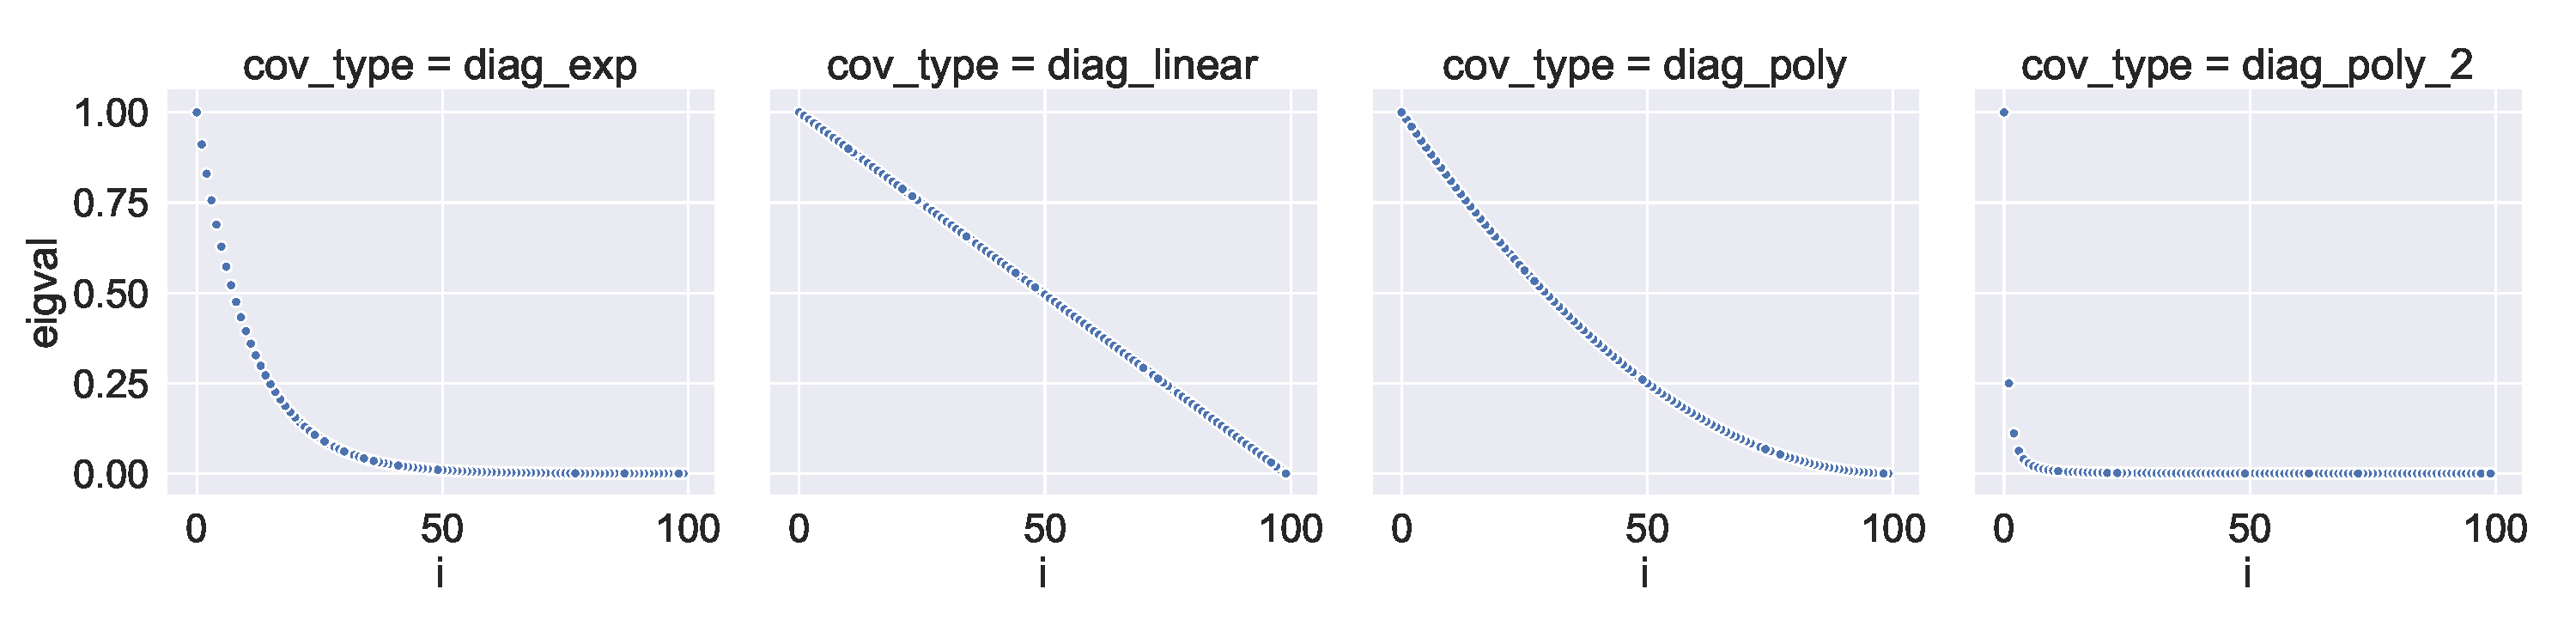
\includegraphics[width=\textwidth]{continuous_figures/decays.pdf}
  \caption{Scree-plots of $\Sigmab$ for the eigenvalue decays examined
    in our empirical valuations. Here $d=100$ for visualization, whereas
    our experiments increase $d$ while preserving the ratio $n/d$ and
    the decay profile,
    with $\lambda_{\text{max}}(\Sigmab) = 1$ to
    $\lambda_{\text{min}}(\Sigmab) = 10^{-4}$.}
  \label{fig:eig-decays}
\end{figure}


We verify our conjectures by incrasing $d$ while keeping the aspect ratio
$n/d$ fixed and examining the rate of decay of the quantities asserted
in the conjectures. As no closed form expressions are available for
the expectations in the conjectures, we estimate $\E\big[\tr(\W^\dagger)\big]$ (for
Conjecture~\ref{c:wishart}) and $\E[\I-\X^\dagger\X]$ (for
Conjecture~\ref{c:projection}) through Monte Carlo sampling. To ensure that
estimation noise is sufficiently small, we continually increase the number
of Monte Carlo samples until the bootstrap confidence intervals are
within $\pm 12.5\%$ of the quantities in \eqref{eq:wishart} and
\eqref{eq:projection}. We found that while
Conjecture~\ref{c:wishart} required a relatively small number of
trials (up to one thousand),
estimation noise was much larger in Conjecture~\ref{c:projection} and
necessitated over two million trials to obtain good estimates
near $d=100$.

% For Conjecture~\ref{c:wishart}, sampling $\W\sim\Wc(\Sigmab,n)$ is
% elementary and the only nontrivial aspect of computing $\Vc(\Sigmab, n)$
% is solving for $\lambda_n$ such that
% $n = \tr(\Sigmab(\Sigmab + \lambda_n \I)^{-1})$. But notice that
% if we let $\tau_i > 0$ be the eigenvalues of $\Sigmab \succ 0$,
% then
% \begin{align*}
%   \tr(\Sigmab(\Sigmab + \lambda \I)^{-1})
%   &= \sum_{i=1}^d \frac{\tau_i}{\tau_i + \lambda}
% \end{align*}
% which is equal to $d > n$ when $\lambda = 0$ and monotonically decreasing in
% $\lambda$. Hence, $\lambda_n$ is unique and can be found using bisection.

\begin{figure}[h]
    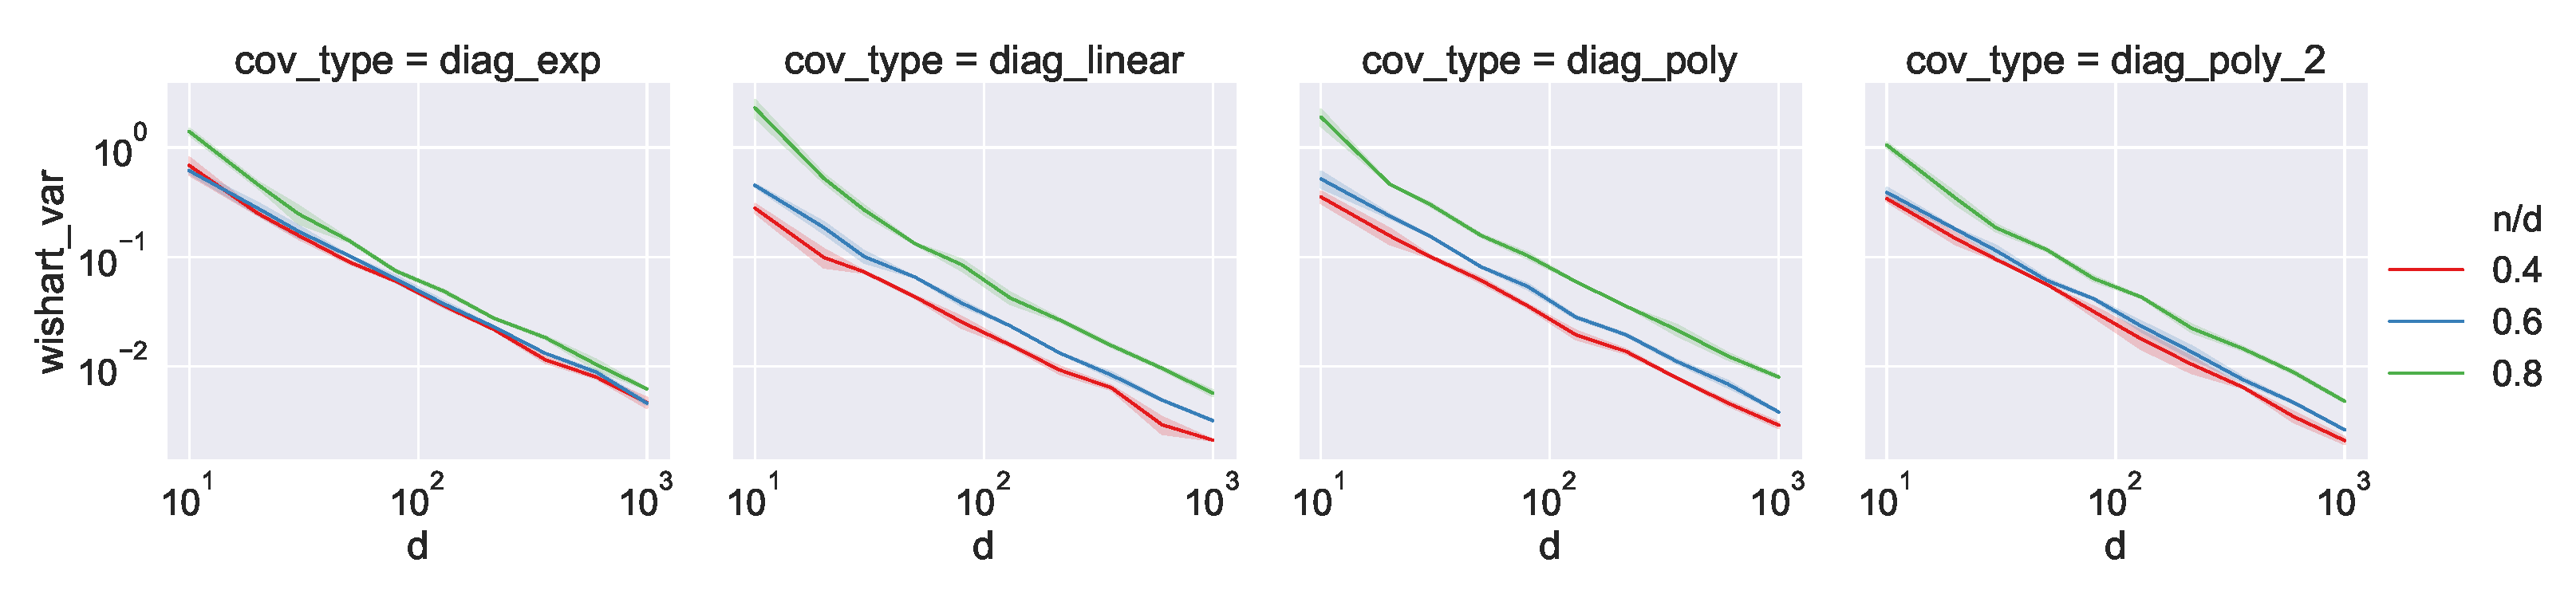
\includegraphics[width=\textwidth]{continuous_figures/wishart_var.pdf}
  \caption{
    Empirical verification of Conjecture~\ref{c:wishart}. We show
    the quantity $\big|\E[\tr(\W^\dagger)]\,\Vc(\Sigmab,n)^{-1} -1\big|$
    as $d$ increases for various aspect ratios $n/d$. Consistent with our conjecture,
    a $O(1/d)$ decay (linear with slope $-1$ on a log-log plot) is
    exhibited across all eigenvalue decay profiles and
    aspect ratios investigated.
  }
  \label{f:conj-wishart}
\end{figure}

The results of empirically validating Conjecture~\ref{c:wishart} are
illustrated in Figure~\ref{f:conj-wishart}, where we performed
Monte Carlo estimation of $\E\big[\tr(\W^\dagger)\big]$ and
plot $\big|\E[\tr(\W^\dagger)]\,\Vc(\Sigmab,n)^{-1} -1\big|$
as $d$ increases from $10$ to $1000$, across a range of aspect ratios $n/d$ and eigenvalue
decay profiles for $\Sigmab$. Confidence intervals are estimated by
bootstrapping. We observe that on log-log axes all of the plots are decreasing with
a linear $-1$ slope, consistent with the $O(1/d)$ rate predicted
by Conjecture~\ref{c:wishart}.


Conjecture \ref{c:projection} is handled similarly, by sampling
$\X\sim\mu^n$ where $\mu=\Nc(\zero,\Sigmab )$ to obtain a Monte Carlo estimate of
$\E[\I-\X^\dagger\X]$. To handle the supremum over $\w$, notice that
we can rewrite \eqref{eq:projection} as a spectral norm
\begin{align}
  \sup_{\w\in\R^d\backslash\{\zero\}}\bigg|\frac{\w^\top\E[\I-\X^\dagger\X]\w}{\w^\top
  \Bc(\Sigmab,n)\w} - 1\bigg|
\  =\ \big\|\E[\I-\X^\dagger\X]\Bc(\Sigmab,n)^{-1}
  - \I\big\|.
  \label{eq:proj-to-operator-norm}
\end{align}
Confidence intervals can now be constructed
using existing methods for constructing operator norm
confidence intervals, and our results use the bootstrapping
method described in \cite{lopes2019bootstrapping}.

Figure~\ref{f:conj-bias} shows
how $\big\|\E[\I-\X^\dagger\X]\Bc(\Sigmab,n)^{-1} - \I\big\|$ decays as we
hold the aspect ratio $n/d$ fixed and increase $d$ between $10$ and
$100$ across the listed
eigenvalue decay profiles and aspect ratios. Again, we observe on
log-log axes a linear decay with slope $-1$ consistent with the $O(1/d)$
rate posed by Conjecture~\ref{c:projection}. Note that the range of
$d$ is smaller than in Figure \ref{f:conj-wishart} because the large
number of Monte Carlo samples (up to two million) required for this
experiment made the computations much more expensive.

\begin{figure}[H]
  \begin{center}
    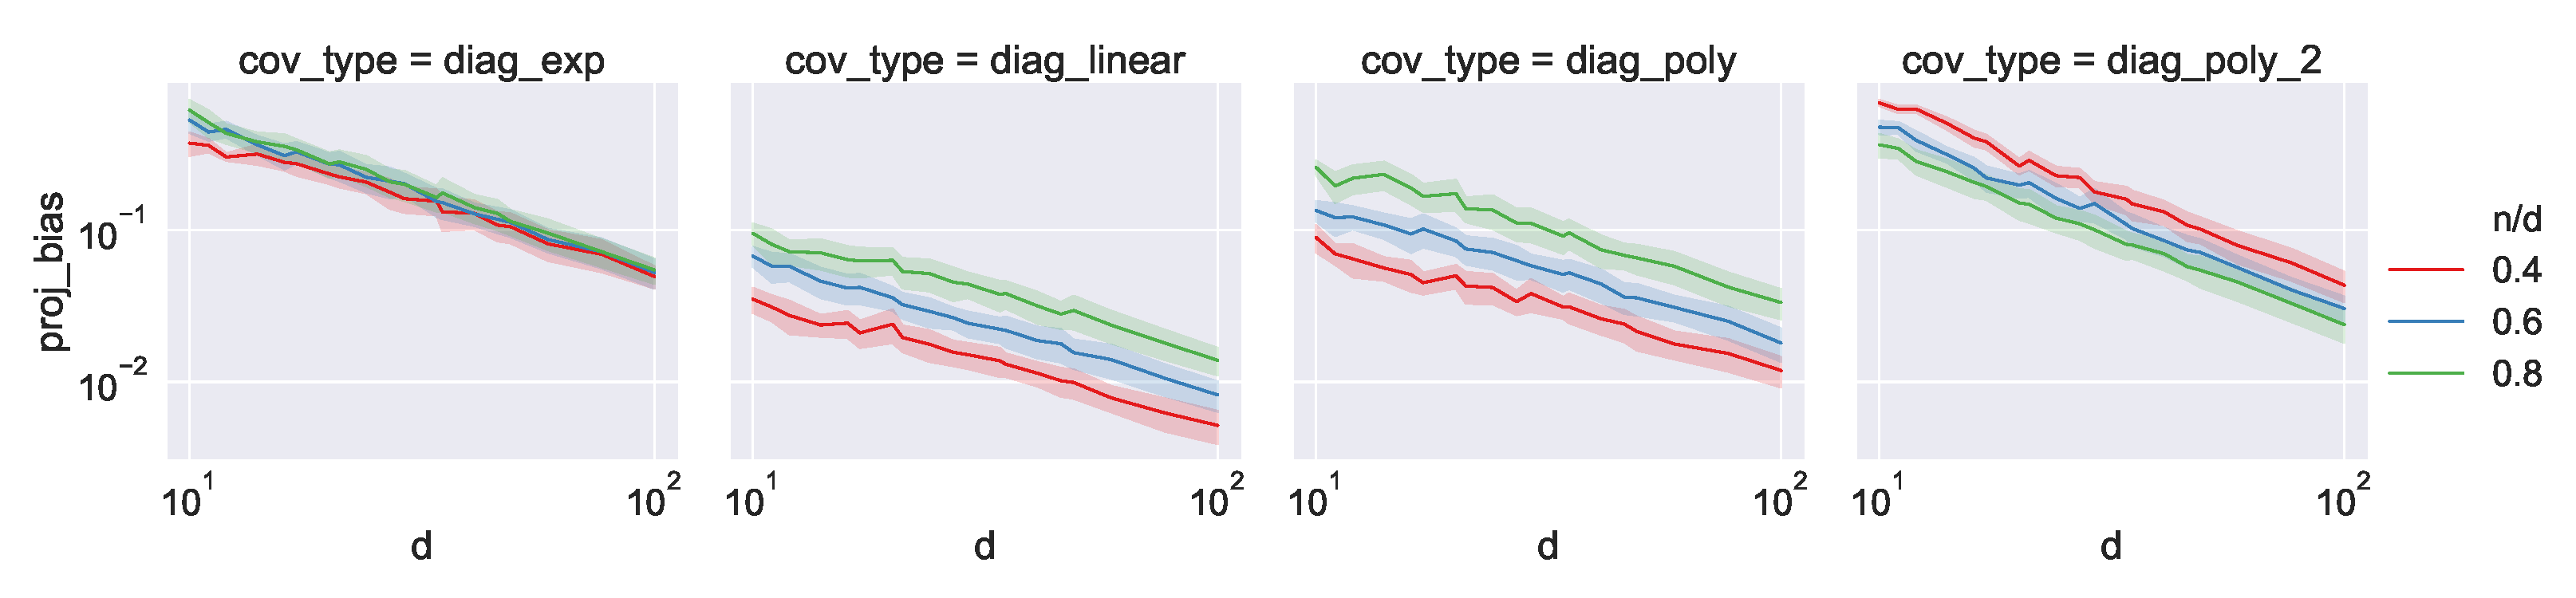
\includegraphics[width=\textwidth]{continuous_figures/proj_bias.pdf}
  \end{center}
  \caption{
    Empirical results validating Conjecture~\ref{c:projection}.
We show how
    $\big\|\E[\I-\X^\dagger\X]\Bc(\Sigmab,n)^{-1} - \I\big\|$
    (which by Equation~\ref{eq:proj-to-operator-norm}
    is equal to the quantity controlled by Conjecture~\ref{c:projection})
    decays as $d$ increases and observe a linear slope consistent with the conjectured $O(1/d)$ rate.
  }
  \label{f:conj-bias}
\end{figure}
